\documentclass{article}

\usepackage{subfigure}

\usepackage{tikz}
\usetikzlibrary{arrows}
\usetikzlibrary{automata}
\usetikzlibrary{calc}
\usetikzlibrary{fit}
\usetikzlibrary{matrix}
\usetikzlibrary{positioning}

\begin{document}

\title{How Fragments Become an NFA:\\ Or, How Sausage is Made}
\maketitle

\begin{figure}
\centering
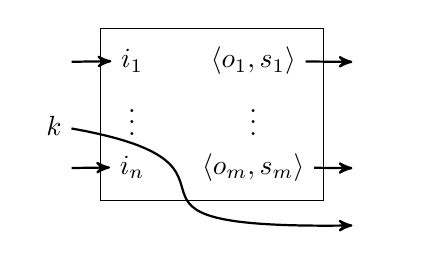
\begin{tikzpicture}

  \matrix [matrix of math nodes,column sep=0.5cm] {
    |(Ato_i_1)| \phantom{x} & |(Ai_1)| i_1 & |(Ao_1)| \langle o_1, s_1 \rangle & |(Afrom_o_1)| \phantom{x} \\
    |(A_k)| k & \vdots & \vdots & \\
    |(Ato_i_n)| \phantom{x} & |(Ai_n)| i_n & |(Ao_m)| \langle o_m, s_m \rangle & |(Afrom_o_m)| \phantom{x} \\[0.25cm]
    &&& |(A_skip)| \phantom{x} \\
  };

  \node [draw,rectangle,fit=(Ai_1) (Ai_n) (Ao_1) (Ao_m)] (A) {};

  \path [draw,thick,->,>=stealth',overlay]
    (Ato_i_1) edge (Ai_1)
    (Ato_i_n) edge (Ai_n)
    (Ao_1)    edge (Afrom_o_1)
    (Ao_m)    edge (Afrom_o_m);

  \path [draw,thick,->,>=stealth',overlay]
    (A_k) .. controls +(-10:3cm) and +($(A_skip) + (170:6cm)$) ..  (A_skip);

\end{tikzpicture}
\caption{An arbitrary fragment}
\end{figure}

\begin{figure}
\centering
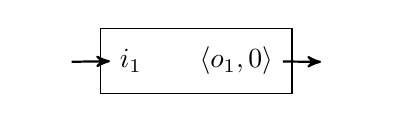
\begin{tikzpicture}

  \matrix [matrix of math nodes,column sep=0.5cm] {
    |(Ato_i_1)| \phantom{x} & |(Ai_1)| i_1 & |(Ao_1)| \langle o_1, 0 \rangle & |(Afrom_o_1)| \phantom{x} \\
  };

  \node [draw,rectangle,fit=(Ai_1) (Ao_1)] (A) {};

  \path [draw,thick,->,>=stealth',overlay]
    (Ato_i_1) edge (Ai_1)
    (Ao_1)    edge (Afrom_o_1);

\end{tikzpicture}
\caption{An atom}
\end{figure}

\begin{figure}
\centering
\subfigure[Greedy]{%
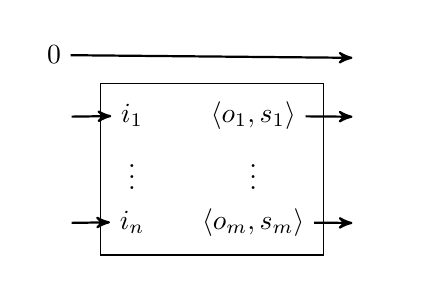
\begin{tikzpicture}

  \matrix [matrix of math nodes,column sep=0.5cm,ampersand replacement=\&] {
    |(A_k)| 0 \&\&\& |(A_skip)| \phantom{x} \\[0.25cm]
    |(Ato_i_1)| \phantom{x} \& |(Ai_1)| i_1 \& |(Ao_1)| \langle o_1, s_1 \rangle \& |(Afrom_o_1)| \phantom{x} \\
    \& \vdots \& \vdots \& \\
    |(Ato_i_n)| \phantom{x} \& |(Ai_n)| i_n \& |(Ao_m)| \langle o_m, s_m \rangle \& |(Afrom_o_m)| \phantom{x} \\
  };

  \node [draw,rectangle,fit=(Ai_1) (Ai_n) (Ao_1) (Ao_m)] (A) {};

  \path [draw,thick,->,>=stealth',overlay]
    (A_k)     edge (A_skip)
    (Ato_i_1) edge (Ai_1)
    (Ato_i_n) edge (Ai_n)
    (Ao_1)    edge (Afrom_o_1)
    (Ao_m)    edge (Afrom_o_m);

\end{tikzpicture}%
}
\subfigure[Nongreedy]{%
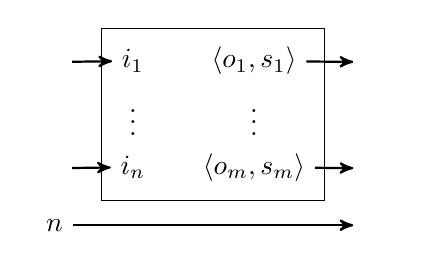
\begin{tikzpicture}

  \matrix [matrix of math nodes,column sep=0.5cm,ampersand replacement=\&] {
    |(Ato_i_1)| \phantom{x} \& |(Ai_1)| i_1 \& |(Ao_1)| \langle o_1, s_1 \rangle \& |(Afrom_o_1)| \phantom{x} \\
    \& \vdots \& \vdots \& \\
    |(Ato_i_n)| \phantom{x} \& |(Ai_n)| i_n \& |(Ao_m)| \langle o_m, s_m \rangle \& |(Afrom_o_m)| \phantom{x} \\[0.25cm]
    |(A_k)| n \&\&\& |(A_skip)| \phantom{x} \\
  };

  \node [draw,rectangle,fit=(Ai_1) (Ai_n) (Ao_1) (Ao_m)] (A) {};

  \path [draw,thick,->,>=stealth',overlay]
    (A_k)     edge (A_skip)
    (Ato_i_1) edge (Ai_1)
    (Ato_i_n) edge (Ai_n)
    (Ao_1)    edge (Afrom_o_1)
    (Ao_m)    edge (Afrom_o_m);

\end{tikzpicture}
}
\caption{Repetition}
\end{figure}













\begin{figure}
\centering
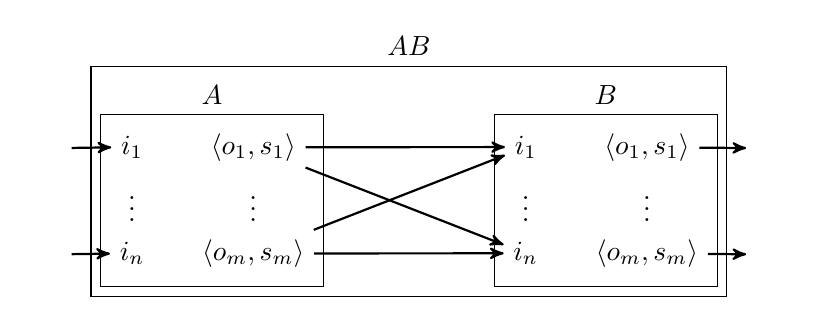
\begin{tikzpicture}

  \matrix [matrix of math nodes,column sep=0.5cm] at (-2.5,0) {
    |(Ato_i_1)| \phantom{x} & |(Ai_1)| i_1 & |(Ao_1)| \langle o_1, s_1 \rangle & |(Afrom_o_1)| \phantom{x} \\
    & \vdots & \vdots & \\
    |(Ato_i_n)| \phantom{x} & |(Ai_n)| i_n & |(Ao_m)| \langle o_m, s_m \rangle & |(Afrom_o_m)| \phantom{x} \\
  };

  \node [draw,rectangle,fit=(Ai_1) (Ai_n) (Ao_1) (Ao_m),label={[name=Alab]above:$A$}] (A) {};

  \path [draw,thick,->,>=stealth',overlay]
    (Ato_i_1) edge (Ai_1)
    (Ato_i_n) edge (Ai_n);

  \matrix [matrix of math nodes,column sep=0.5cm] at (2.5,0) {
    |(Bto_i_1)| \phantom{x} & |(Bi_1)| i_1 & |(Bo_1)| \langle o_1, s_1 \rangle & |(Bfrom_o_1)| \phantom{x} \\
    & \vdots & \vdots & \\
    |(Bto_i_n)| \phantom{x} & |(Bi_n)| i_n & |(Bo_m)| \langle o_m, s_m \rangle & |(Bfrom_o_m)| \phantom{x} \\
  };

  \node [draw,rectangle,fit=(Bi_1) (Bi_n) (Bo_1) (Bo_m),label={[name=Blab]above:$B$}] (B) {};

  \path [draw,thick,->,>=stealth',overlay]
    (Bo_1) edge (Bfrom_o_1)
    (Bo_m) edge (Bfrom_o_m);

  \path [draw,thick,->,>=stealth']
    (Ao_1) edge (Bi_1)
    (Ao_1) edge (Bi_n)
    (Ao_m) edge (Bi_1)
    (Ao_m) edge (Bi_n);

  \node [draw,rectangle,fit=(A) (Alab) (B) (Blab),label=above:$AB$] (AB) {};

\end{tikzpicture}
\caption{Concatenation: $A.k = B.k = \emptyset$}
\end{figure}

\begin{figure}
\centering
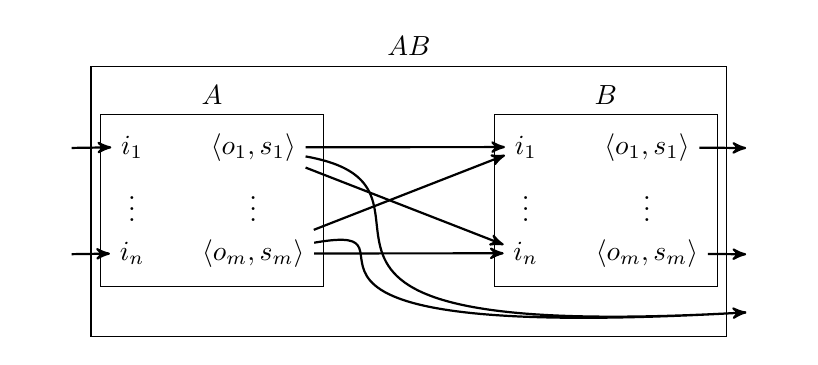
\begin{tikzpicture}

  \matrix [matrix of math nodes,column sep=0.5cm,anchor=north] at (-2.5,0) {
    |(Ato_i_1)| \phantom{x} & |(Ai_1)| i_1 & |(Ao_1)| \langle o_1, s_1 \rangle & |(Afrom_o_1)| \phantom{x} \\
    & \vdots & \vdots & \\
    |(Ato_i_n)| \phantom{x} & |(Ai_n)| i_n & |(Ao_m)| \langle o_m, s_m \rangle & |(Afrom_o_m)| \phantom{x} \\
  };

  \node [draw,rectangle,fit=(Ai_1) (Ai_n) (Ao_1) (Ao_m),label={[name=Alab]above:$A$}] (A) {};

  \path [draw,thick,->,>=stealth',overlay]
    (Ato_i_1) edge (Ai_1)
    (Ato_i_n) edge (Ai_n);

  \matrix [matrix of math nodes,column sep=0.5cm,anchor=north] at (2.5,0) {
    |(Bto_i_1)| \phantom{x} & |(Bi_1)| i_1 & |(Bo_1)| \langle o_1, s_1 \rangle & |(Bfrom_o_1)| \phantom{x} \\
    & \vdots & \vdots & \\
    |(Bto_i_n)| \phantom{x} & |(Bi_n)| i_n & |(Bo_m)| \langle o_m, s_m \rangle & |(Bfrom_o_m)| \phantom{x} \\[0.25cm]
    && |(B_skip)| & |(Bfrom_skip)| \phantom{x} \\
  };

  \node [draw,rectangle,fit=(Bi_1) (Bi_n) (Bo_1) (Bo_m),label={[name=Blab]above:$B$}] (B) {};

  \path [draw,thick,->,>=stealth',overlay]
    (Bo_1) edge (Bfrom_o_1)
    (Bo_m) edge (Bfrom_o_m);

  \path [draw,thick,->,>=stealth']
    (Ao_1) edge (Bi_1)
    (Ao_1) edge (Bi_n)
    (Ao_m) edge (Bi_1)
    (Ao_m) edge (Bi_n);

  \path [draw,thick,->,>=stealth',overlay]
    (Ao_1) .. controls +(-10:3cm) and +($(Bfrom_skip) + (170:12cm)$) .. (Bfrom_skip)
    (Ao_m) .. controls +(10:2.5cm) and +($(Bfrom_skip) + (170:12cm)$) .. (Bfrom_skip);


  \node [draw,rectangle,fit=(A) (Alab) (B) (Blab) (B_skip),label=above:$AB$] (AB) {};

\end{tikzpicture}
\caption{Concatenation: $A.k = \emptyset, B.k \ne \emptyset$}
\end{figure}

\begin{figure}
\centering
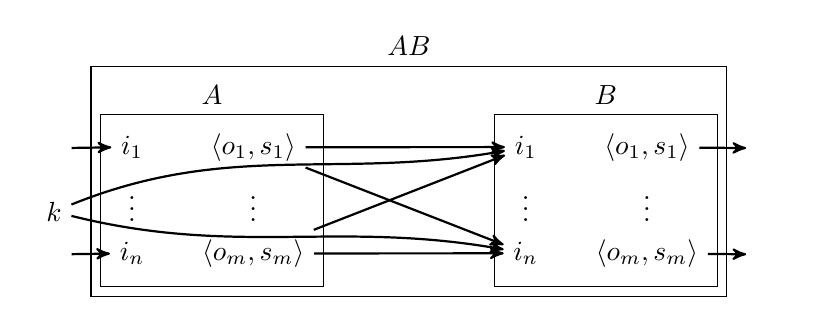
\begin{tikzpicture}

  \matrix [matrix of math nodes,column sep=0.5cm] at (-2.5,0) {
    |(Ato_i_1)| \phantom{x} & |(Ai_1)| i_1 & |(Ao_1)| \langle o_1, s_1 \rangle & |(Afrom_o_1)| \phantom{x} \\
    |(A_skip)| k & \vdots & \vdots & \\
    |(Ato_i_n)| \phantom{x} & |(Ai_n)| i_n & |(Ao_m)| \langle o_m, s_m \rangle & |(Afrom_o_m)| \phantom{x} \\
  };

  \node [draw,rectangle,fit=(Ai_1) (Ai_n) (Ao_1) (Ao_m),label={[name=Alab]above:$A$}] (A) {};

  \path [draw,thick,->,>=stealth',overlay]
    (Ato_i_1) edge (Ai_1)
    (Ato_i_n) edge (Ai_n);

  \matrix [matrix of math nodes,column sep=0.5cm] at (2.5,0) {
    |(Bto_i_1)| \phantom{x} & |(Bi_1)| i_1 & |(Bo_1)| \langle o_1, s_1 \rangle & |(Bfrom_o_1)| \phantom{x} \\
    & \vdots & \vdots & \\
    |(Bto_i_n)| \phantom{x} & |(Bi_n)| i_n & |(Bo_m)| \langle o_m, s_m \rangle & |(Bfrom_o_m)| \phantom{x} \\
  };

  \node [draw,rectangle,fit=(Bi_1) (Bi_n) (Bo_1) (Bo_m),label={[name=Blab]above:$B$}] (B) {};

  \path [draw,thick,->,>=stealth',overlay]
    (Bo_1) edge (Bfrom_o_1)
    (Bo_m) edge (Bfrom_o_m);

  \path [draw,thick,->,>=stealth']
    (Ao_1) edge (Bi_1)
    (Ao_1) edge (Bi_n)
    (Ao_m) edge (Bi_1)
    (Ao_m) edge (Bi_n);

  \node [draw,rectangle,fit=(A) (Alab) (B) (Blab),label=above:$AB$] (AB) {};

  \path [draw,thick,->,>=stealth',overlay]
    (A_skip) edge [out=22,in=190] (Bi_1)
    (A_skip) edge [out=-14,in=170] (Bi_n);

\end{tikzpicture}
\caption{Concatenation: $A.k \ne \emptyset, B.k = \emptyset$}
\end{figure}

\begin{figure}
\centering
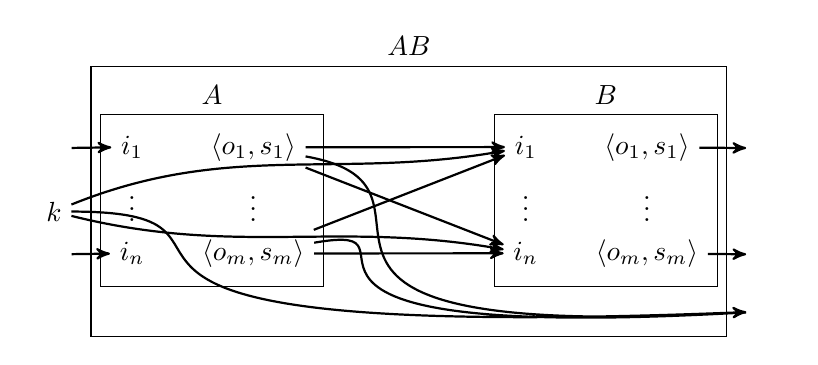
\begin{tikzpicture}

  \matrix [matrix of math nodes,column sep=0.5cm,anchor=north] at (-2.5,0) {
    |(Ato_i_1)| \phantom{x} & |(Ai_1)| i_1 & |(Ao_1)| \langle o_1, s_1 \rangle & |(Afrom_o_1)| \phantom{x} \\
    |(A_skip)| k & \vdots & \vdots & \\
    |(Ato_i_n)| \phantom{x} & |(Ai_n)| i_n & |(Ao_m)| \langle o_m, s_m \rangle & |(Afrom_o_m)| \phantom{x} \\
  };

  \node [draw,rectangle,fit=(Ai_1) (Ai_n) (Ao_1) (Ao_m),label={[name=Alab]above:$A$}] (A) {};

  \path [draw,thick,->,>=stealth',overlay]
    (Ato_i_1) edge (Ai_1)
    (Ato_i_n) edge (Ai_n);

  \matrix [matrix of math nodes,column sep=0.5cm,anchor=north] at (2.5,0) {
    |(Bto_i_1)| \phantom{x} & |(Bi_1)| i_1 & |(Bo_1)| \langle o_1, s_1 \rangle & |(Bfrom_o_1)| \phantom{x} \\
    & \vdots & \vdots & \\
    |(Bto_i_n)| \phantom{x} & |(Bi_n)| i_n & |(Bo_m)| \langle o_m, s_m \rangle & |(Bfrom_o_m)| \phantom{x} \\[0.25cm]
    && |(B_skip)| & |(Bfrom_skip)| \phantom{x} \\
  };

  \node [draw,rectangle,fit=(Bi_1) (Bi_n) (Bo_1) (Bo_m),label={[name=Blab]above:$B$}] (B) {};

  \path [draw,thick,->,>=stealth',overlay]
    (Bo_1) edge (Bfrom_o_1)
    (Bo_m) edge (Bfrom_o_m);

  \path [draw,thick,->,>=stealth']
    (Ao_1) edge (Bi_1)
    (Ao_1) edge (Bi_n)
    (Ao_m) edge (Bi_1)
    (Ao_m) edge (Bi_n);

  \node [draw,rectangle,fit=(A) (Alab) (B) (Blab) (B_skip),label=above:$AB$] (AB) {};

  \path [draw,thick,->,>=stealth',overlay]
    (A_skip) edge [out=22,in=190] (Bi_1)
    (A_skip) edge [out=-14,in=170] (Bi_n);

  \path [draw,thick,->,>=stealth',overlay]
    (Ao_1) .. controls +(-10:3cm) and +($(Bfrom_skip) + (170:12cm)$) .. (Bfrom_skip)
    (Ao_m) .. controls +(10:2.5cm) and +($(Bfrom_skip) + (170:12cm)$) .. (Bfrom_skip)
    (A_skip) .. controls +(0:3.25cm) and +($(Bfrom_skip) + (172:15cm)$) .. (Bfrom_skip);

\end{tikzpicture}
\caption{Concatenation: $A.k \ne \emptyset, B.k \ne \emptyset$}
\end{figure}

\begin{figure}
\centering
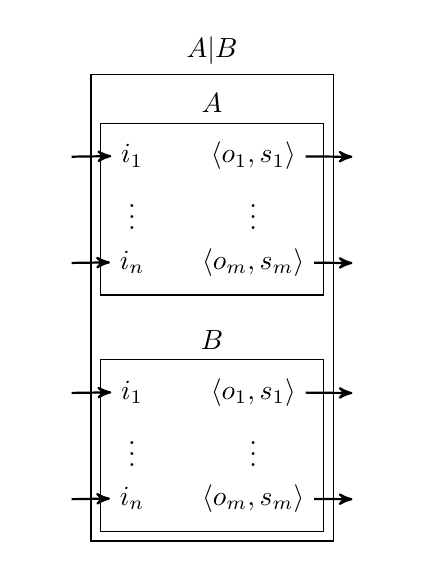
\begin{tikzpicture}

  \matrix [matrix of math nodes,column sep=0.5cm] at (0,1.5) {
    |(Ato_i_1)| \phantom{x} & |(Ai_1)| i_1 & |(Ao_1)| \langle o_1, s_1 \rangle & |(Afrom_o_1)| \phantom{x} \\
    & \vdots & \vdots & \\
    |(Ato_i_n)| \phantom{x} & |(Ai_n)| i_n & |(Ao_m)| \langle o_m, s_m \rangle & |(Afrom_o_m)| \phantom{x} \\
  };

  \node [draw,rectangle,fit=(Ai_1) (Ai_n) (Ao_1) (Ao_m),label={[name=Alab]above:$A$}] (A) {};

  \path [draw,thick,->,>=stealth',overlay]
    (Ato_i_1) edge (Ai_1)
    (Ato_i_n) edge (Ai_n)
    (Ao_1)    edge (Afrom_o_1)
    (Ao_m)    edge (Afrom_o_m);

  \matrix [matrix of math nodes,column sep=0.5cm] at (0,-1.5) {
    |(Bto_i_1)| \phantom{x} & |(Bi_1)| i_1 & |(Bo_1)| \langle o_1, s_1 \rangle & |(Bfrom_o_1)| \phantom{x} \\
    & \vdots & \vdots & \\
    |(Bto_i_n)| \phantom{x} & |(Bi_n)| i_n & |(Bo_m)| \langle o_m, s_m \rangle & |(Bfrom_o_m)| \phantom{x} \\
  };

  \node [draw,rectangle,fit=(Bi_1) (Bi_n) (Bo_1) (Bo_m),label={[name=Blab]above:$B$}] (B) {};

   \path [draw,thick,->,>=stealth',overlay]
    (Bto_i_1) edge (Bi_1)
    (Bto_i_n) edge (Bi_n)
    (Bo_1)    edge (Bfrom_o_1)
    (Bo_m)    edge (Bfrom_o_m);

  \node [draw,rectangle,fit=(A) (Alab) (B) (Blab),label=above:$A|B$] (AB) {};

\end{tikzpicture}
\caption{Alternation: $A.k = B.k = \emptyset$}
\end{figure}

\begin{figure}
\centering
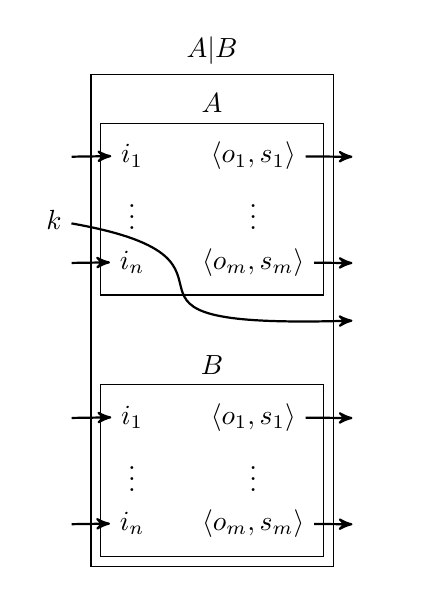
\begin{tikzpicture}

  \matrix [matrix of math nodes,column sep=0.5cm] at (0,1.5) {
    |(Ato_i_1)| \phantom{x} & |(Ai_1)| i_1 & |(Ao_1)| \langle o_1, s_1 \rangle & |(Afrom_o_1)| \phantom{x} \\
    |(A_k)| k & \vdots & \vdots & \\
    |(Ato_i_n)| \phantom{x} & |(Ai_n)| i_n & |(Ao_m)| \langle o_m, s_m \rangle & |(Afrom_o_m)| \phantom{x} \\[0.25cm]
    &&& |(A_skip)| \phantom{x} \\
  };

  \node [draw,rectangle,fit=(Ai_1) (Ai_n) (Ao_1) (Ao_m),label={[name=Alab]above:$A$}] (A) {};

  \path [draw,thick,->,>=stealth',overlay]
    (Ato_i_1) edge (Ai_1)
    (Ato_i_n) edge (Ai_n)
    (Ao_1)    edge (Afrom_o_1)
    (Ao_m)    edge (Afrom_o_m);

  \path [draw,thick,->,>=stealth',overlay]
    (A_k) .. controls +(-10:3cm) and +($(A_skip) + (185:6cm)$) ..  (A_skip);

  \matrix [matrix of math nodes,column sep=0.5cm] at (0,-1.5) {
    |(Bto_i_1)| \phantom{x} & |(Bi_1)| i_1 & |(Bo_1)| \langle o_1, s_1 \rangle & |(Bfrom_o_1)| \phantom{x} \\
    & \vdots & \vdots & \\
    |(Bto_i_n)| \phantom{x} & |(Bi_n)| i_n & |(Bo_m)| \langle o_m, s_m \rangle & |(Bfrom_o_m)| \phantom{x} \\
  };

  \node [draw,rectangle,fit=(Bi_1) (Bi_n) (Bo_1) (Bo_m),label={[name=Blab]above:$B$}] (B) {};

   \path [draw,thick,->,>=stealth',overlay]
    (Bto_i_1) edge (Bi_1)
    (Bto_i_n) edge (Bi_n)
    (Bo_1)    edge (Bfrom_o_1)
    (Bo_m)    edge (Bfrom_o_m);

  \node [draw,rectangle,fit=(A) (Alab) (B) (Blab),label=above:$A|B$] (AB) {};

\end{tikzpicture}
\caption{Alternation: $A.k \ne \emptyset$}
\end{figure}

\begin{figure}
\centering
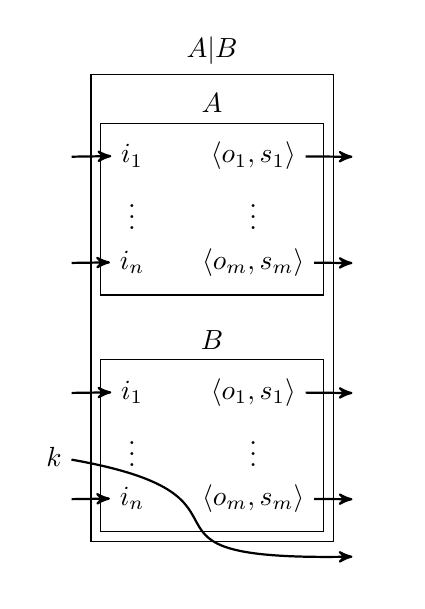
\begin{tikzpicture}

  \matrix [matrix of math nodes,column sep=0.5cm] at (0,1.5) {
    |(Ato_i_1)| \phantom{x} & |(Ai_1)| i_1 & |(Ao_1)| \langle o_1, s_1 \rangle & |(Afrom_o_1)| \phantom{x} \\
    & \vdots & \vdots & \\
    |(Ato_i_n)| \phantom{x} & |(Ai_n)| i_n & |(Ao_m)| \langle o_m, s_m \rangle & |(Afrom_o_m)| \phantom{x} \\[0.25cm]
    &&& |(A_skip)| \phantom{x} \\
  };

  \node [draw,rectangle,fit=(Ai_1) (Ai_n) (Ao_1) (Ao_m),label={[name=Alab]above:$A$}] (A) {};

  \path [draw,thick,->,>=stealth',overlay]
    (Ato_i_1) edge (Ai_1)
    (Ato_i_n) edge (Ai_n)
    (Ao_1)    edge (Afrom_o_1)
    (Ao_m)    edge (Afrom_o_m);

  \matrix [matrix of math nodes,column sep=0.5cm] at (0,-1.5) {
    |(Bto_i_1)| \phantom{x} & |(Bi_1)| i_1 & |(Bo_1)| \langle o_1, s_1 \rangle & |(Bfrom_o_1)| \phantom{x} \\
    |(B_k)| k & \vdots & \vdots & \\
    |(Bto_i_n)| \phantom{x} & |(Bi_n)| i_n & |(Bo_m)| \langle o_m, s_m \rangle & |(Bfrom_o_m)| \phantom{x} \\[0.25cm]
    &&& |(B_skip)| \phantom{x} \\
  };

  \node [draw,rectangle,fit=(Bi_1) (Bi_n) (Bo_1) (Bo_m),label={[name=Blab]above:$B$}] (B) {};

   \path [draw,thick,->,>=stealth',overlay]
    (Bto_i_1) edge (Bi_1)
    (Bto_i_n) edge (Bi_n)
    (Bo_1)    edge (Bfrom_o_1)
    (Bo_m)    edge (Bfrom_o_m);

  \path [draw,thick,->,>=stealth',overlay]
    (B_k) .. controls +(-10:3cm) and +($(B_skip) + (155:6cm)$) .. (B_skip);

  \node [draw,rectangle,fit=(A) (Alab) (B) (Blab),label=above:$A|B$] (AB) {};

\end{tikzpicture}
\caption{Alternation: $A.k = \emptyset, B.k \ne \emptyset$}
\end{figure}

\end{document}
